\documentclass{article}
\usepackage{graphicx}
\usepackage[margin=1.5cm]{geometry}
\usepackage{amsmath}

\begin{document}
\twocolumn

\title{Monday Warm Up: Unit 5: Momentum II}
\author{Prof. Jordan C. Hanson}

\maketitle

\section{Memory Bank}

\begin{itemize}
\item $v = r \omega$ ... Relationship between tangential velocity and angular velocity.
\item $\omega = 2\pi f = 2\pi/T$ ... Relationship between angular velocity ($\omega$), frequency ($f$), and period ($T$).
\item $\vec{p} = m\vec{v}$ ... Definition of momentum.
\item $\vec{F}_{\rm Net} = \frac{d\vec{p}}{dt}$ ... Force and momentum
\item Let $M$ be the total mass of a system, and let $m_j$ and $\vec{r}_j$ $(j = 1,...,N)$ be the masses and positions of the constituent parts of the system.  The position of the center of mass is
\begin{equation}
\vec{r}_{\rm CM} = \frac{1}{M}\sum_{j=1}^{N}m_j \vec{r}_j
\end{equation}
\item The momentum of the center of mass $\vec{P}_{\rm CM}$ is
\begin{equation}
\vec{P}_{\rm CM} = \sum_{j=1}^N \vec{p}_j
\end{equation}
\item The net external force on a system obeys
\begin{equation}
\vec{F} = \frac{d\vec{P}_{\rm CM}}{dt}
\end{equation}
\end{itemize}

\section{Momentum II}

\begin{enumerate}
\item In Pre-columbian and colonial period Latin America, \textit{gauchos} would sometimes hunt with a weapons known as \textit{bolas} (Fig. \ref{fig:1}).  The bolas were thrown, and would spin around the center of mass until they wrapped the limbs of the prey. (a) Suppose two masses $m$ are separated by a diameter $d$.  The positions of the masses are $r_1(t) = \frac{1}{2}d\cos(2\pi f t)$ and $r_2(t) = \frac{1}{2}d\cos(2\pi f t-\pi)$.  (a) Graph the positions in an x-y coordinate system.  (b) Locate the center of mass at $t = 0$. (c) Suppose $f = 5$ Hz, or 5 rotations per second.  Locate the center of mass at $t=0.2$ seconds. \\ \vspace{3cm}
\item Consider the same bola system as the previous exercise.  (a) If the frequency $f$ is 5 Hz, what is the angular velocity? (b) What is the tangential velocity of each bola, if $d = 0.7$ m?  (c) If the mass of each bola is 1.2 kg, and the bolas are following $r_1(t)$ and $r_2(t)$, what is the magnitude of the momentum of each bola?  (d) What is the \textit{total momentum} $P_{\rm CM}$? \\ \vspace{2cm}
\item Now suppose the gaucho throws the bola (Fig. \ref{fig:1}), and the \textit{center of mass} has an initial velocity of 20 m s$^{-1}$ at a 45 degree angle.  (a) How far does it travel before it lands?  (b) Does the rotation of the bolas around the center of mass affect how far it goes? \\ \vspace{2cm}
\end{enumerate}

\begin{figure}[hb]
\centering
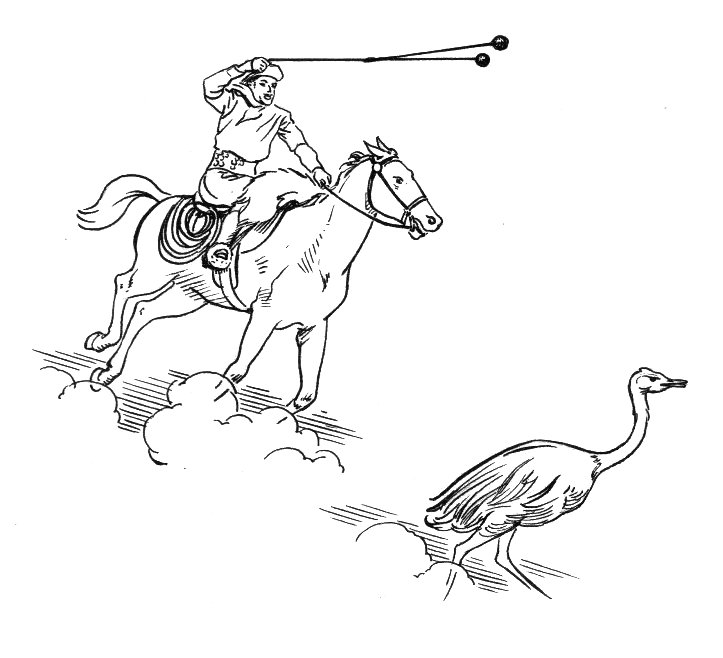
\includegraphics[width=0.4\textwidth]{figures/Bola.jpg}
\caption{\label{fig:1} A \textit{gaucho} using a bola weapon to hunt a rhea bird.}
\end{figure}

\end{document}
